\subsection{Results and Discussion}
% -------------------------------------------------------------------------
This section compares the in-situ x-radiography, the backscattered
electron images, and calculations from solidification theory and discusses
how the methods viewed together provide more context about the material
when viewed together than each of the methods would provide on their own.

\subsubsection{In Situ x-Radiography}
% -------------------------------------------------------------------------
A subset of the sequence of processed x-radiographs presented shows the
solidifying Al-rich dendrites and the progressively Ag-enriched liquid
(\ref{fig/03/rad-seq}). Light and dark pixel intensities correspond
to the Al-rich and Ag-enriched regions, respectively.

\begin{figure}[ht]
    \centering
    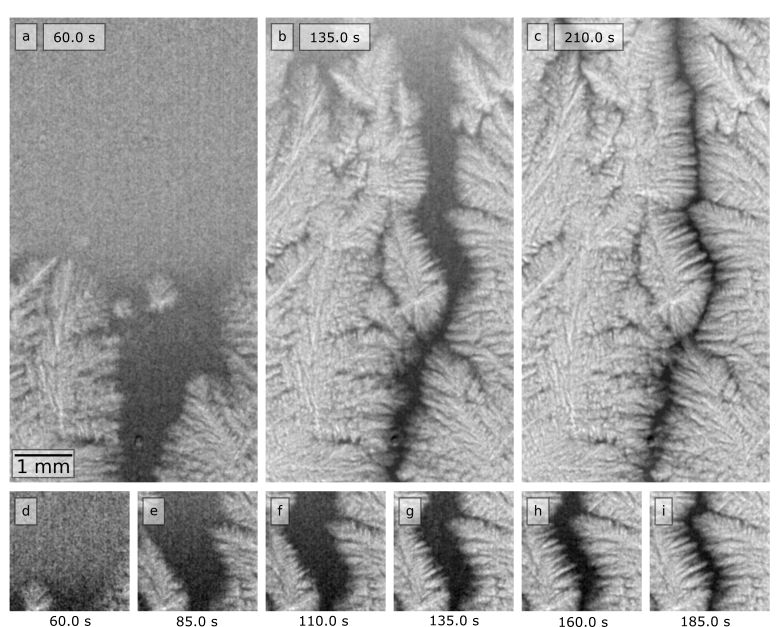
\includegraphics[width=0.6\textwidth]{figures/03/01-rad-seq.png}
    \caption{
        \small\setstretch{1}
        (a - c) In situ x-radiographs showing the mesoscale solidification of
        an Al-9.68 Ag at.\% sample, with time shown in seconds passed since the
        start of solidification within the viewing window.
        (d - i) Additional frames for a region of interest in the middle
        right of the full sample. Lighter regions are Al-rich, whereas darker
        regions are Ag-rich.
    }
    \label{fig/03/rad-seq}
\end{figure}

% -------------------------------------------------------------------------
\subsubsection{Backscattered Electron Image Comparison}
% -------------------------------------------------------------------------
Multiple post-solidification BSE images were used to create a single BSE
image montage for comparison with the x-radiography data at the end of
solidification (Fig. \ref{fig/03/sem-rad}).
Because BSE signal intensity increases with Z \cite{Reuter2003},
regions of high Ag concentrations are represented by lighter areas in the
image, while darker areas represent low Ag concentrations. This being the
case, it is reasonable to conclude that the small pits observed in very
light regions inherited high Ag contents (e.g., from enriched
interdendritic liquid) relative to their surroundings, leading to
corrosion during polishing. In the radiographs, the intensity relationship
is reversed because regions of high Ag decrease the transmission of
x-rays, resulting in darker pixels. Despite differences in spatial
resolution and signal depth between these two techniques, the BSE images
(\ref{fig/03/sem-rad}.a, b) are perceived as inverted relative to the
x-radiography (as expected). To allow for a clearer comparison,
an inverted BSE image is included (\ref{fig/03/sem-rad}.c)
to show the similarities in the solidified features
with the fully solidified x-radiograph (\ref{fig/03/sem-rad}.d).
This observation highlights the fact that Z values have a strong influence on
contrast in x-radiography.

\begin{figure}[ht]
    \centering
    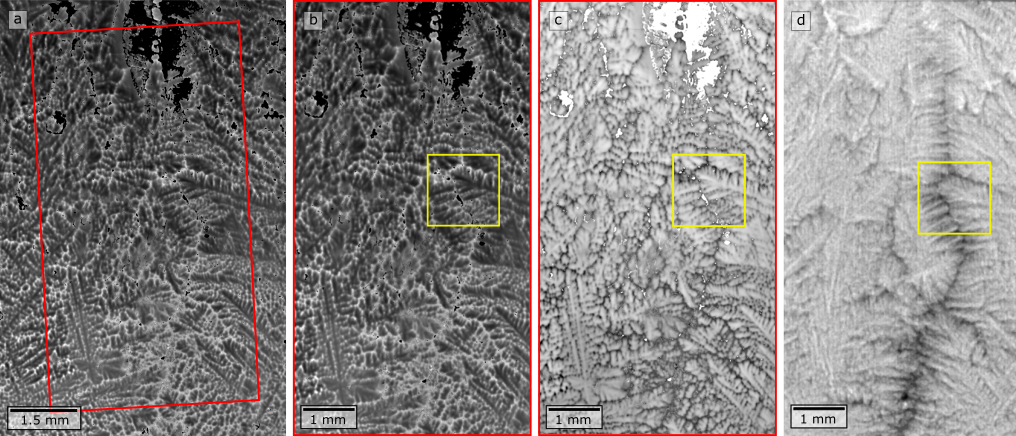
\includegraphics[width=0.6\textwidth]{figures/03/02-sem-rad.png}
    \caption{
        \small\setstretch{1}
        (a) Post-solidification BSE image montage with the area of the
        sample analyzed through in situ x-radiography indicated by the red
        overlay.
        (b) BSE image rotated and cropped to the x-radiography analysis
        area with the yellow overlay corresponding to the region of interest in
        \ref{fig/03/rad-seq}.d - i.
        (c) BSE image with grayscale values inverted to facilitate
        visual comparison to x-radiography with the region of interest once
        again indicated by the yellow overlay.
        (d) X-radiograph of the fully solidified
        sample (939 s after the start of solidification). Yellow overlay
        corresponds to the same region of interest as in (b) and (c).
    }
    \label{fig/03/sem-rad}
\end{figure}

% -------------------------------------------------------------------------
\subsubsection{Solidification Calculation Comparison}
% -------------------------------------------------------------------------
Following the frame progression during solidification in
\ref{fig/03/rad-seq}.d - i, the first solid to form is a light-colored
dendrite. According to the phase diagram (\ref{fig/03/sem-rad}.a),
this primary solid is expected to have a low Ag
content, which causes the interdendritic fluid to become enriched with Ag.
As solidification continues, Ag concentrations in both the recently frozen
solid and the remaining liquid increase as the Al-rich solid continues to
partition Ag into the liquid. The Scheil solidification model is shown and
compared with the evolution of the fraction of phases using an equilibrium
(lever rule) solidification path (\ref{fig/03/sem-rad}.b).

\begin{figure}[ht]
    \centering
    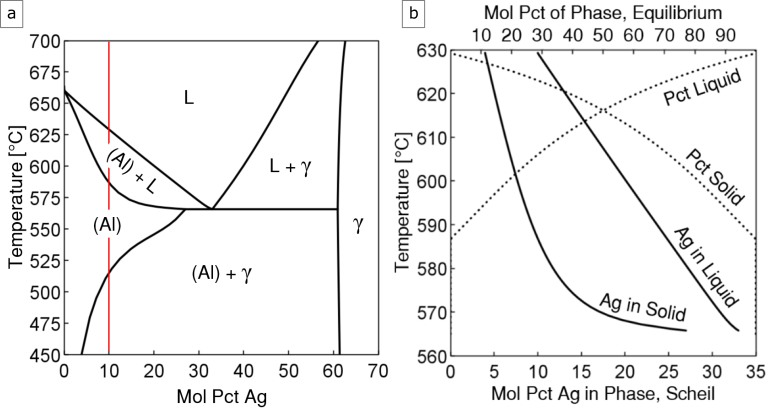
\includegraphics[width=0.6\textwidth]{figures/03/03-phase-scheil.png}
    \caption{
        \small\setstretch{1}
        (a) An equilibrium Al-Ag phase diagram with the sample composition
        (Al-9.68 Ag at.\%) indicated by a red line.
        (b) Thermo-Calc solidification calculations showing Ag concentrations
        in the liquid and solid phases (Scheil, solid lines) and phase
        percentages (Equilibrium, dotted lines).
    }
    \label{fig/03/phase-scheil}
\end{figure}

In the Scheil calculation results (\ref{fig/03/phase-scheil}.b),
as expected from the phase
diagram, Ag concentration is found to increase for both the liquid and
solid phases during solidification, and the solidus temperature is reduced
from the equilibrium value of 587°C to the eutectic temperature at around
566°C, as indicated by the ends of the Scheil curves (solid lines)
compared to the equilibrium fractions (dotted lines). At this temperature,
the Scheil model indicates that the remaining liquid reaches the eutectic
point (33 mole percent Ag) and solidifies as an (Al + $\gamma$) microconstituent.
The trend of progressive Ag enrichment in the liquid phase is consistent
with the BSE images and x-radiographs.

The results obtained from the Scheil calculations can also be compared
directly to the radiographs by measuring the fraction solidified at
different times during solidification. Using Python, solid regions were
identified and manually labeled by tracing the solid structures on label
layers in the napari image viewer. This created binary mask images which
were overlaid on each other to show the progression of the solidification.
These binary masks were then analyzed using the measure submodule of
scikit-image to compare the area solidified of each image to the total
area of the images. At this point, the as-measured fraction solid, with
each image representing different solidification temperatures, was
compared to the Scheil simulation results expressed as fraction solid and
temperature. By aligning the as-measured fraction solid with the Scheil
calculated fraction solid, a mapping was made from solidification
temperature (position in image sequence) to solid composition
(\ref{fig/03/solid-frac}.a).
The measurement of fraction solid does not continue for the full range of
solidification because the solidification occurred slowly at the end of
the experiment, so the best fitting portion of the Scheil simulation also
does not reach complete solidification. This image number to solid
composition mapping from the Scheil simulation at any given instant was
then used to estimate the concentration of the solid formed between two
successive radiographs, ultimately constructing a spatiotemporal solute
microsegregation map (\ref{fig/03/solid-frac}.b).

\begin{figure}[ht]
    \centering
    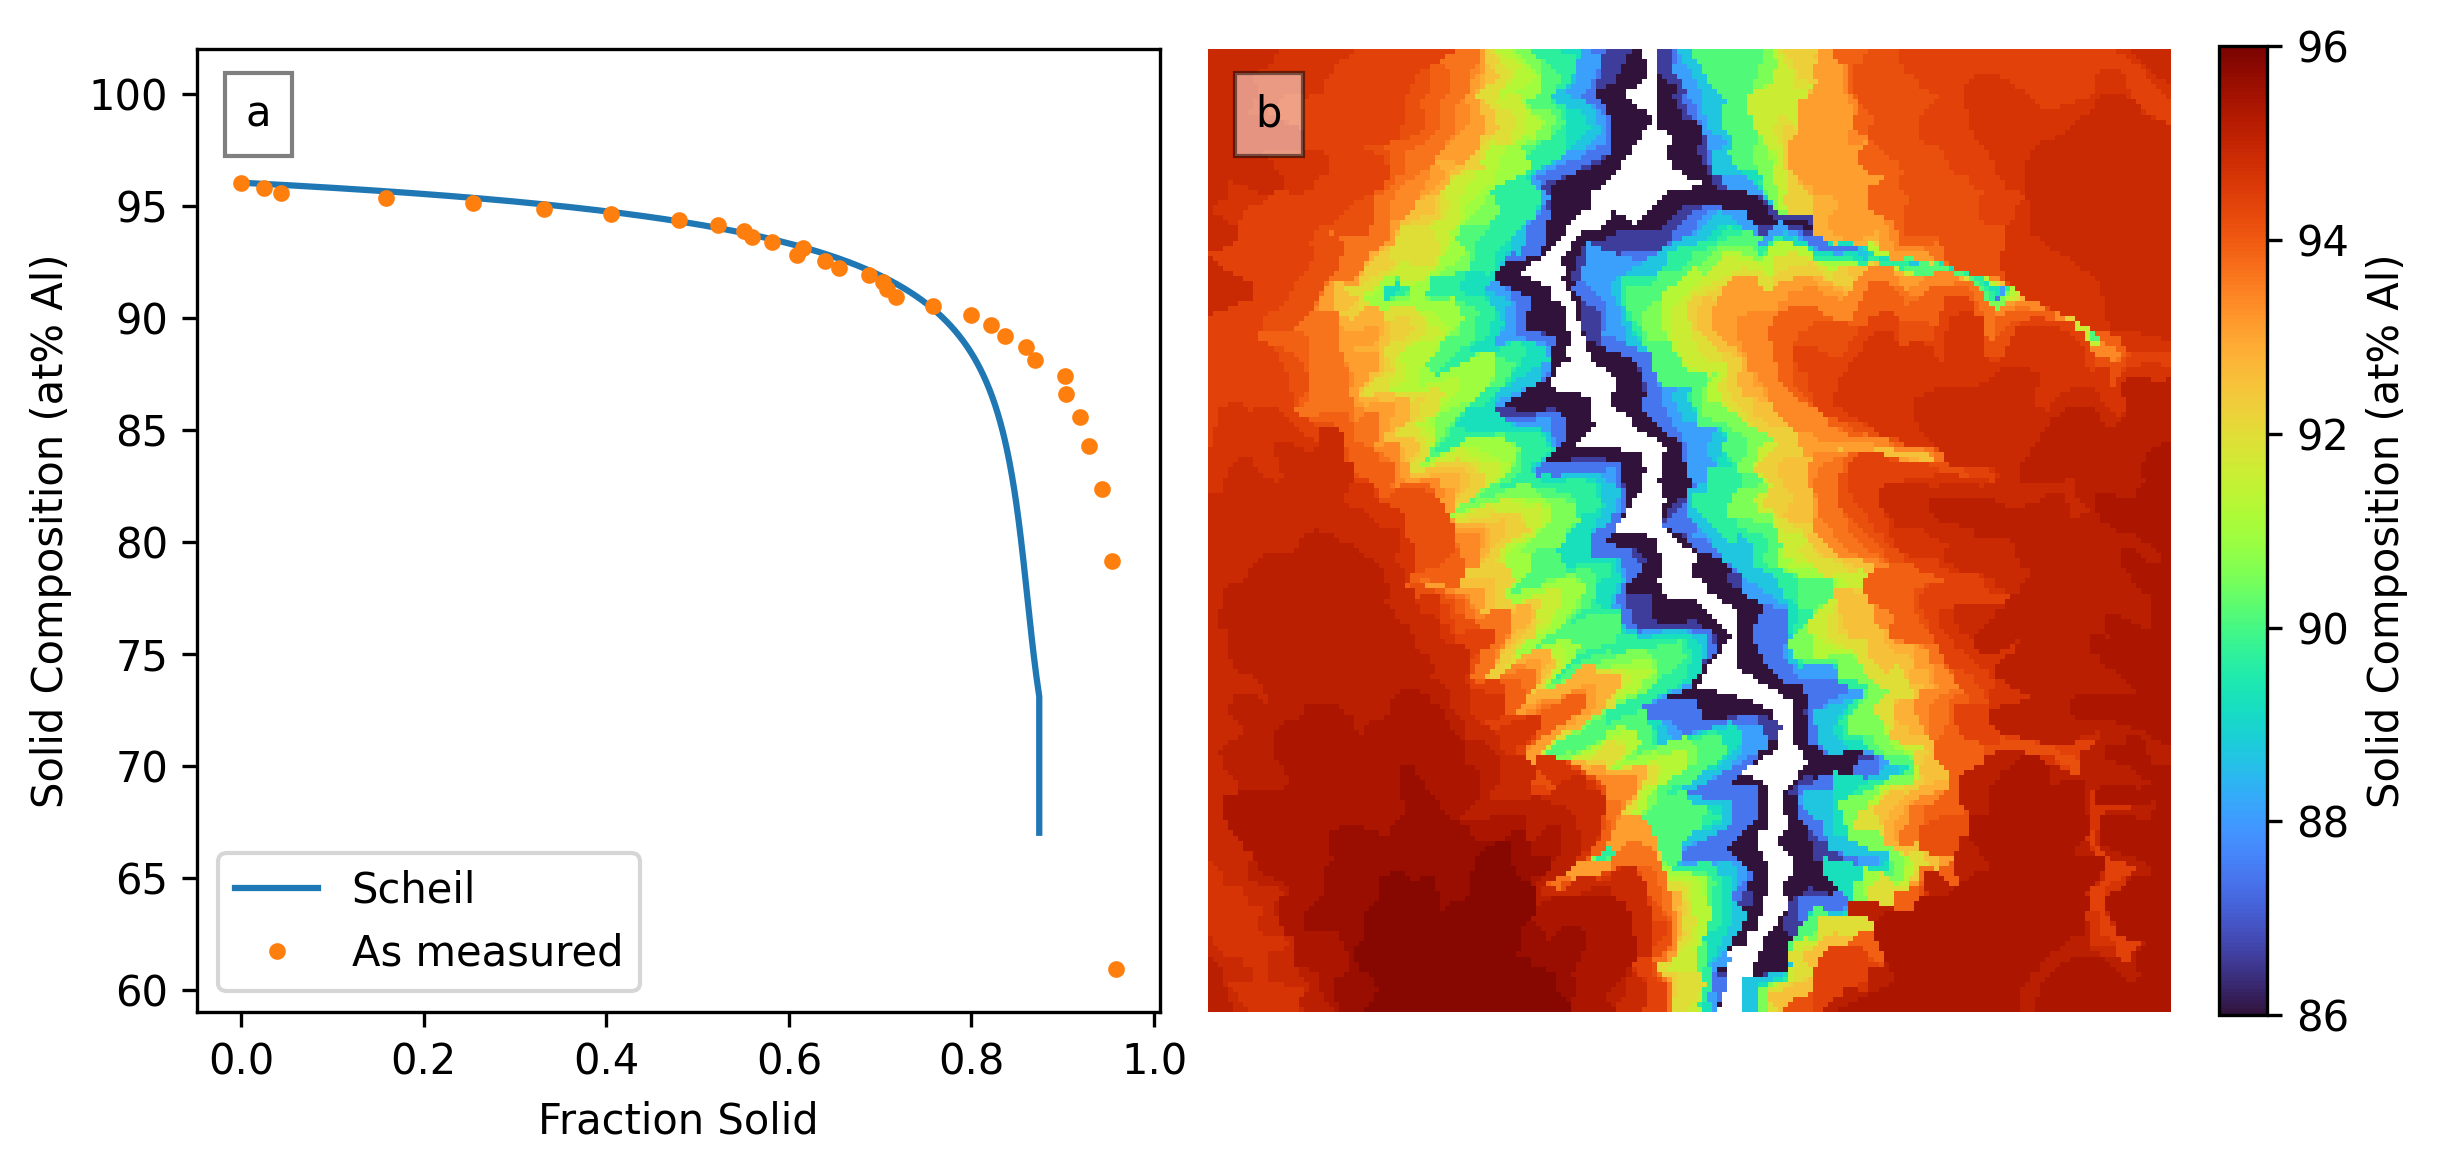
\includegraphics[width=0.6\textwidth]{figures/03/04-solid-frac.png}
    \caption{
        \small\setstretch{1}
        (a) Comparison between the Scheil solidification simulation results
        expressed as solid composition versus fraction solid (blue) and the
        Scheil solid composition data mapped to the fraction solid as measured
        in this region of the radiographs (orange).
        (b) Mapping fraction solid to composition of the solid at the point
        of solidification (at\% Al) during in situ x-radiography. Color
        represents decreasing Al content of the solid forming during
        solidification.
    }
    \label{fig/03/solid-frac}
\end{figure}

Using this matching procedure between Scheil simulation results and
radiographs, which is based on the observable solid fraction, the
agreement between simulation and experiments lead to a good match
(\ref{fig/03/solid-frac}.a) for most of the freezing range, with some
deviation at high solid fraction.
This is directly due to a discrepancy in solid fraction between
model and experiments: given the underlying assumption that the cooling
rate is homogeneous and constant, temperature (simulation) and time
(x-radiography) axes are thus kept linear with respect to each other,
which in turn results in the deviation in fraction versus composition
estimation at high solid fraction (\ref{fig/03/solid-frac}.a).
This discrepancy could, to
some extent, be addressed by relaxing the assumption of homogeneous and
constant cooling rate, allowing it to deviate from this ideal case locally
(in time and space), for instance, by directly using the concentration
versus solid fraction curve from the CalPhaD calculation to estimate the
concentration profile (instead of the solid fraction versus time and/or
temperature). Another possible source of error stems from how the fraction
solid was measured in the radiographs. Since the x-rays travel through the
entire volume of the sample, liquid trapped between dendrites or dendrites
that form but do not span the entire thickness of the sample could be
measured as a fully solid area, even though they represent a volume that
may not be completely solid. Additionally, only a single region of
interest of the sample is analyzed in this way, so it is also possible
that this region is not completely representative, as some solute may
enter and exit this region to other portions of the sample, and
temperature may also vary beyond this region. While the current 2D
analysis already provides a reasonable estimation of the solid fraction,
it might be further enhanced using contrast-based volumetric
reconstruction through the sample.35 An important feature of the
microsegregation analysis technique proposed here is that, while
approximate and relying on strong assumption (e.g., CalPhaD-based
solidification path), it is straightforward to extend to multicomponent
solute mapping. This would be impossible to obtain through radiography
analysis alone and could provide an important tool for further analysis of
time-dependent in situ imaging data.

% -------------------------------------------------------------------------
\subsubsection{Comparing EDS and x-Radiography}
% -------------------------------------------------------------------------
Comparisons between the EDS-determined compositions and the radiograph
intensities can be made, despite differences in the techniques for
collecting these datasets. These comparisons were made by using Python and
the napari image viewer to manually overlay the BSE montage image, the
individual BSE images containing the overlay of the line scan locations,
and the x-radiograph showing the fully solidified structure. With these
images aligned, a line could be placed on the x-radiography in the
location corresponding to the EDS line scan, such that the corresponding
pixel intensity of the x-radiograph could be determined. While pixel
intensities in x-radiography convey information about composition due to
varying Z of the material in the sample, the intensities also convey
information about the entire thickness of the sample. This is contrasted
with the volume sampled by EDS, which is only on the order of 3 µm from
the metallographically prepared surface (approximately 30 µm below the
surface of the as-solidified sample). Since this volume is about two orders
of magnitude smaller than the volume probed by x-radiography
(already the small approximately 250 µm thickness), the EDS is more akin to
an analysis of the surface. These differences need to be considered when
comparing the data. A comparison of an EDS line scan showing the Al content
over the length of the line shows similar trends to the x-ray intensity
profile of a line in the same location on the aligned radiograph
(\ref{fig/03/eds-vs-rad-1}).

\begin{figure}[ht]
    \centering
    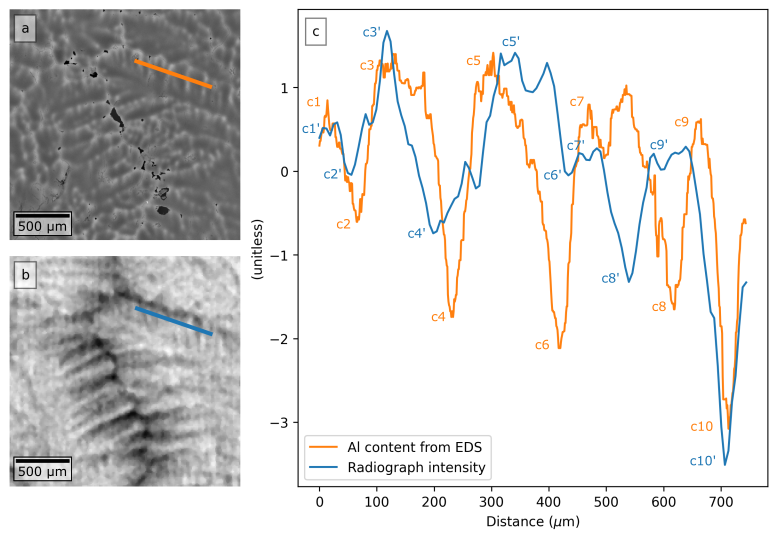
\includegraphics[width=0.6\textwidth]{figures/03/05-eds-vs-rad-01-09.png}
    \caption{
        \small\setstretch{1}
        (a) BSE image of an Al-Ag sample showing the position of an EDS
        line scan measuring the Al content.
        (b) X-radiograph of the same sample region, post-solidification.
        (c) Al content from the EDS line scan (orange) and the transmitted
        x-ray intensity (blue), collected across the length of the lines in
        (a) and (b) respectively. Each dataset is standardized to a unitless
        range for comparison. EDS features annotated as c1 - 10 correlate to
        x-radiography features annotated as c1' - 10', respectively.
    }
    \label{fig/03/eds-vs-rad-1}
\end{figure}

Annotations along the datasets in \ref{fig/03/eds-vs-rad-1}.c show
features consistent across
the length of the line across the sample for both EDS and radiography. The
line is oriented such that the beginning is near the tip of a primary
dendrite, traveling along the secondary dendrite arms towards the areas
that were first to solidify. Many correlated features exist between these
datasets, such as the maxima annotated in \ref{fig/03/eds-vs-rad-1}.c
as c1 and c1', c3 and
c3', and c5 and c5', and the minima annotated as c10 and c10'. Differences
between the datasets can be reasonably explained considering the nature of
the acquisition techniques. One way these discrepancies could manifest is
through local maxima or minima in the datasets not centered at the same
location along the lines. Volume measurements captured by x-radiography
are expected to deviate from the surface measurements captured by EDS in
the case when a given feature in the sample (e.g., a secondary dendrite
arm) may not be oriented in a way that places its center of volume
directly in line with the cross-section measured at the surface by EDS.

Another manifestation of the discrepancies that arise due to the
differences in volume versus surface effects of these two modes of
analysis is considered in the region of the sample analyzed across
well-defined secondary dendrite arms (\ref{fig/03/eds-vs-rad-2}).
The EDS and radiograph profile data is normalized in the same way as in
\ref{fig/03/eds-vs-rad-1}, and, although we
see correlations between the minima and maxima of the datasets, the
general trend across the entire length of the EDS data exhibits maxima and
minima (corresponding to Al-rich dendritic and Ag-rich interdendritic
regions, respectively) at similar intensities
(orange line, \ref{fig/03/eds-vs-rad-2}.c). In
contrast, the x-radiography intensity (blue line) progressively increases
across the length of the line.

\begin{figure}[ht]
    \centering
    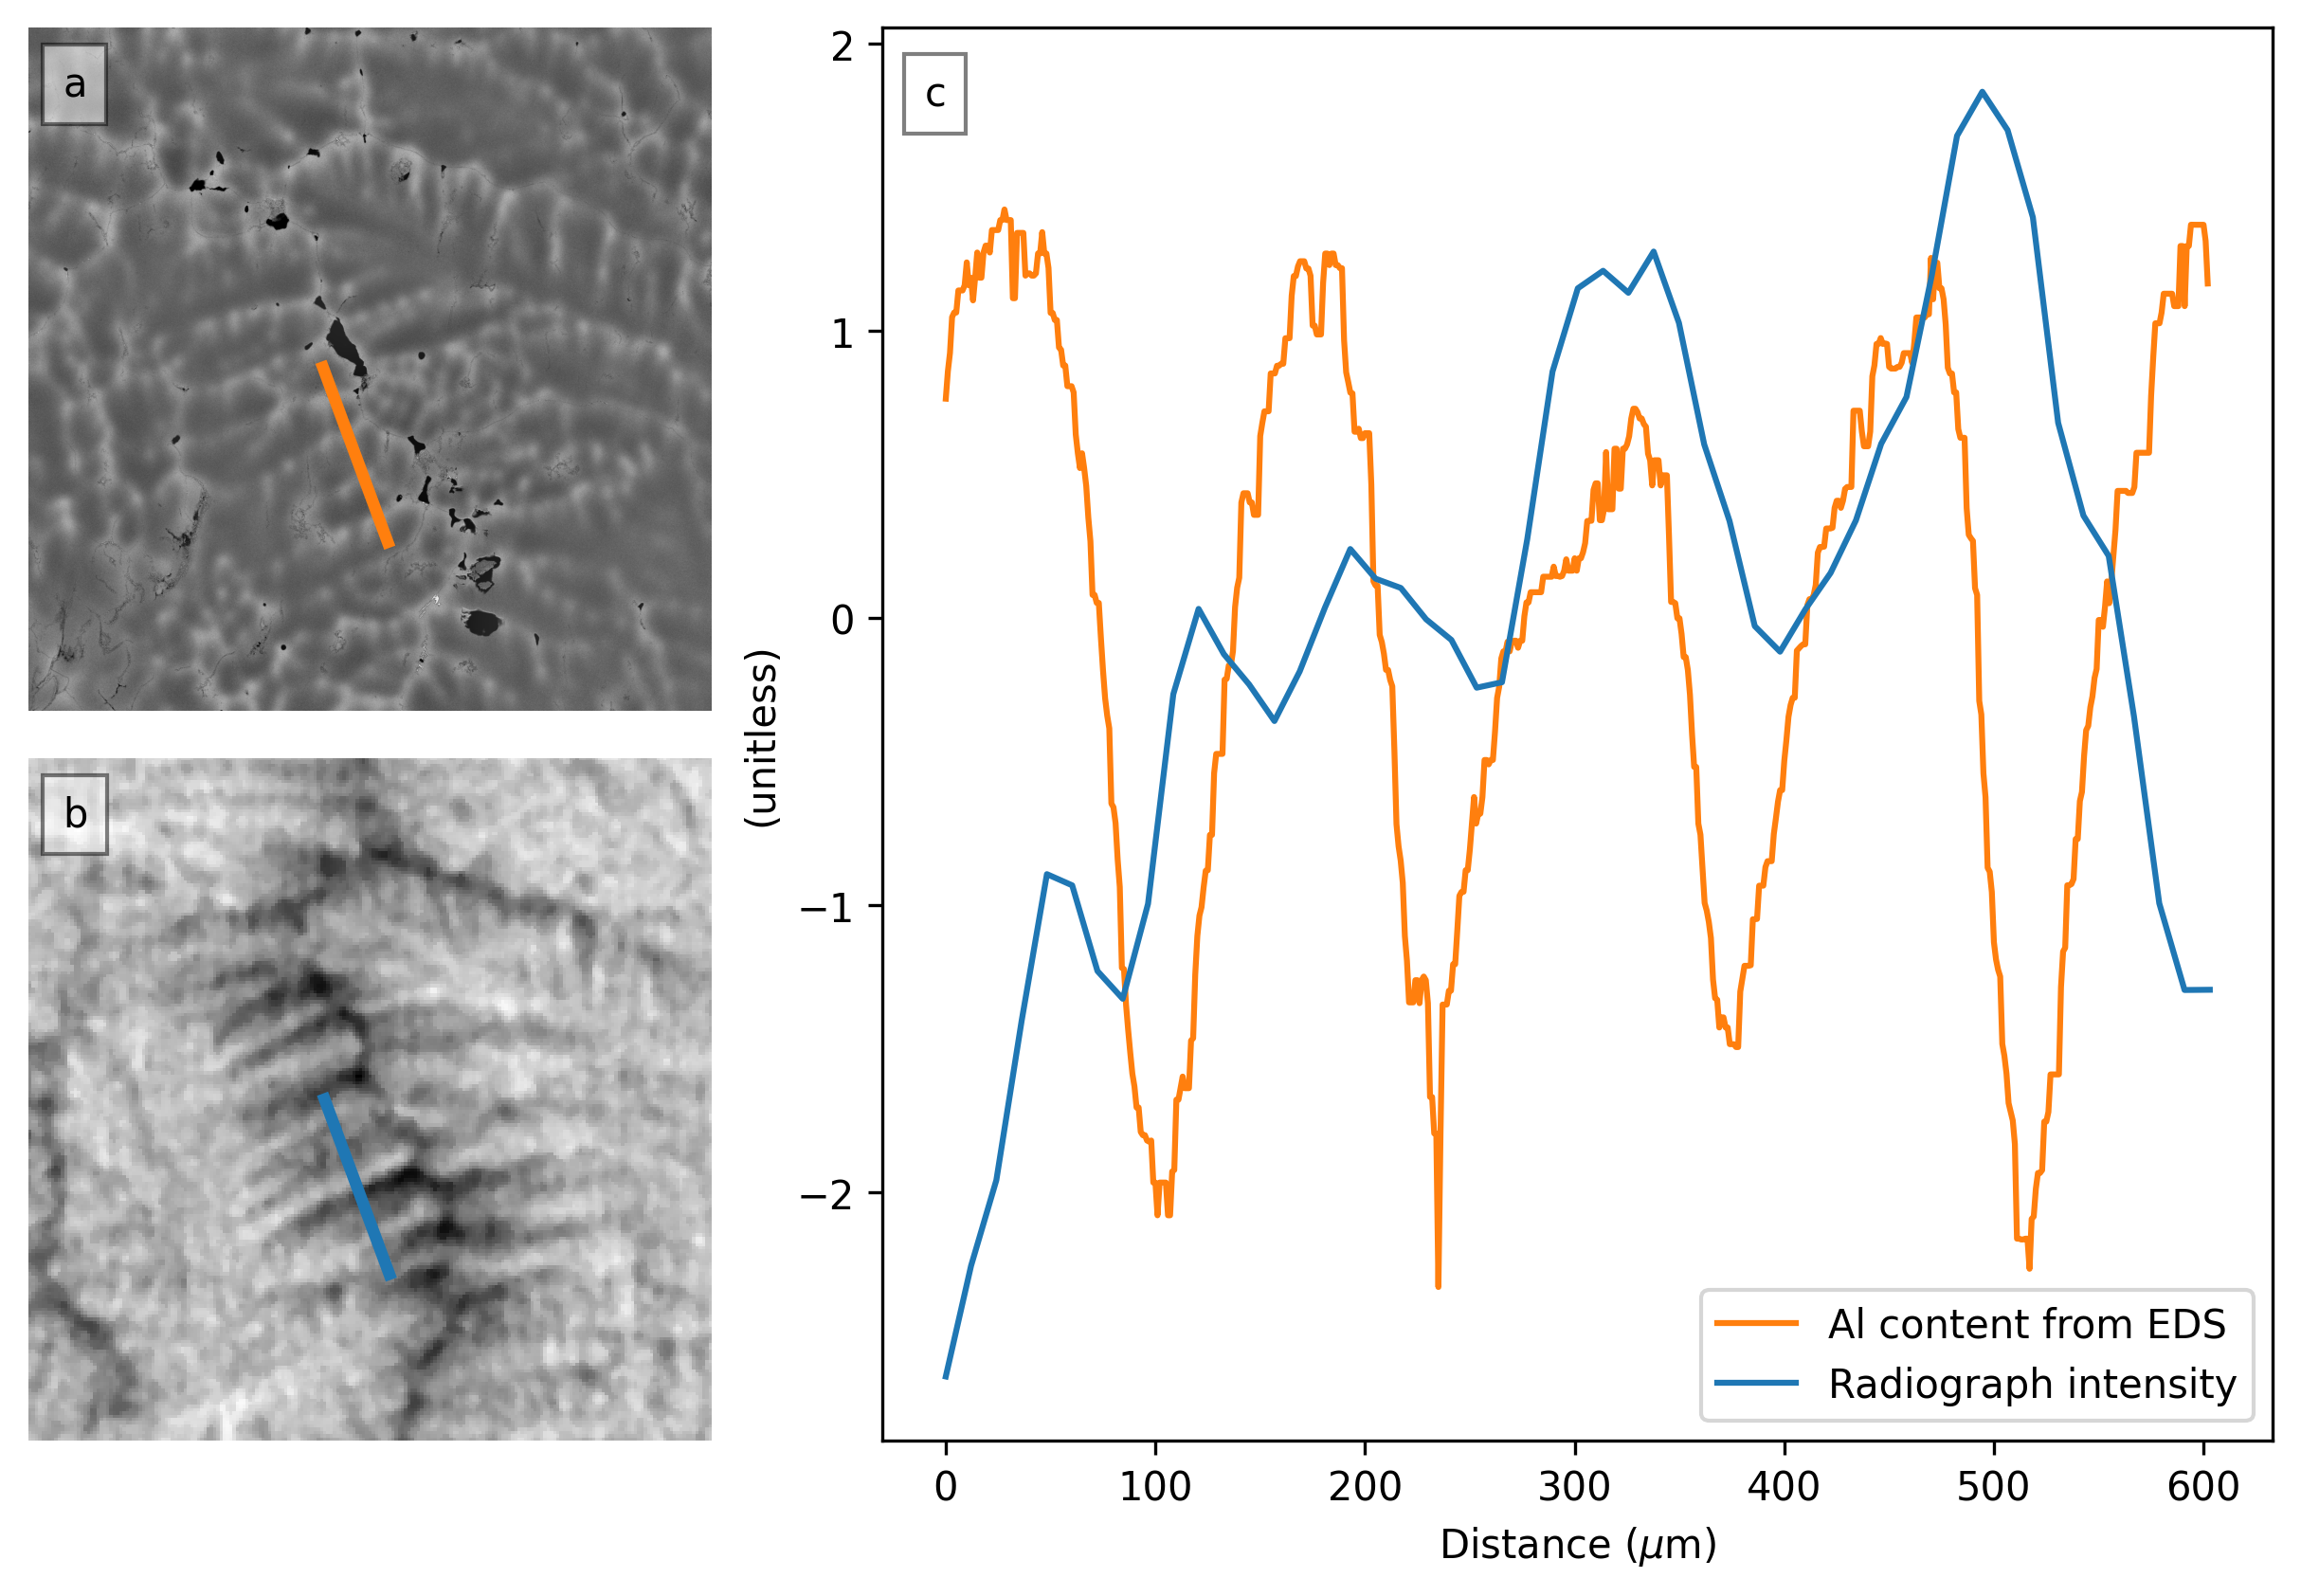
\includegraphics[width=0.6\textwidth]{figures/03/06-eds-vs-rad-05-17-1.png}
    \caption{
        \small\setstretch{1}
        (a) BSE image of an Al-Ag sample showing the position of an EDS
        line scan measuring the Al content.
        (b) X-radiograph of the same sample region, post-solidification.
        (c) Al content from the EDS line scan (orange) and the transmitted
        x-ray intensity from the x-radiograph (blue). Each dataset was
        standardized to a unitless range for comparison, with data collected
        across the length of the lines in (a) and (b), starting at the top
        left endpoint of the line and moving towards the bottom center of
        the images.
    }
    \label{fig/03/eds-vs-rad-2}
\end{figure}

One possibility for this discrepancy could be the decreasing thickness of
the dendrite arms along the length of the line, rather than composition
differences. Progressively increasing intensity in x-radiography data
corresponds to progressively higher transmission of x-rays. Hence, the
secondary dendrite arms further along the length of the line of analysis
could be progressively thinner, allowing for more x-rays to be
transmitted. This may not be visible at the surface after solidification
is complete (and therefore would not show in the EDS data). Even if the
dendrite arms were the same size and shape, differing orientations with
respect to each other could still cause the dendrite arms to have more
volume in the path of the x-rays.

Another possibility that may explain some mismatch between the datasets is
the existence of multiple layers of dendrites or of sidebranches within
the sample thickness. In the annotations of
Fig. \ref{fig/03/eds-vs-rad-2}.c, most of the features
of the EDS data are seen to correlate with the x-radiography, except for
the feature annotated as c3. In the radiography, c3' consists of two
separate peaks, whereas, in the EDS, what we see can be considered a
higher single peak (with some noise). Possibly, a secondary dendrite arm
between the two EDS maxima c1 and c3, but below the surface, such that it
would be behind these other two surface dendrites, could lead to this
additional local maximum in the radiography data, whereas it would remain
undetectable from surface analysis. When we compare the areas around the
length of the line on the SEM image (Fig. \ref{fig/03/eds-vs-rad-2}.a) and
the radiograph (\ref{fig/03/eds-vs-rad-2}.b),
we see the correlation between dendrite arms c1 and c1'; however, the
interdendritic region c2 and the following dendrite arm c3 are clear in
the EDS data, but neither c2' nor c3' is clear in the radiograph.
Solid-state diffusion is another possibility to alter the compositions of
the final, as-solidified microstructure measured by EDS, relative to those
that exist just after solidification and observed by radiography.

While direct comparisons between x-radiography and EDS remain challenging,
especially due to differences arising between the volume-probing nature of
x-radiography and the surface analysis nature of EDS, the combination of
these characterization methods enables relative changes during materials
processing to be analyzed in a laboratory setting. Three-dimensional
analysis, such as 3D computed tomography, could be considered as an
additional concurrent data source, which would support or discard such
interpretations of through-thickness features in the sample. Future work
and some of the potential exploration pathways deriving from this work are
briefly mentioned in the following section.

% -------------------------------------------------------------------------
\subsubsection{Perspectives}
% -------------------------------------------------------------------------
Combining both in situ and post-solidification diagnostics, as well as
modeling and simulation tools, offers many exploration pathways for
ongoing and future work. Using CalPhaD alone, several ways of
reconstructing the microsegregation profile may be envisioned, only one of
which has been illustrated here. Frameworks may be considered that would
for instance combine (1) compositional analysis directly from the
gray-level radiographs
\cite{Ruvalcaba2007,Bogno2011,Bogno2013,Becker2016a,Becker2020,Mirihanage2014}
(however, limited to binary alloys
for a semi-quantitative analysis), (2) microsegregation simulations using
different approaches, such as lever rule, Gulliver-Scheil, or models
accounting for finite diffusivities (e.g., using CalPhaD-based or other
volume-averaged methods \cite{Tourret2009}), and
(3) further post-solidification
compositional analyses, such as wavelength dispersive spectroscopy, the
amount of redundancy with EDS possibly being used as a cross-validation
tool or for more comprehensive analysis.

Combining in situ imaging data and simulations also provides numerous
promising avenues for data analysis of transient conditions during
solidification, and determination of physical parameters otherwise
extremely challenging to estimate, if measurable at all. One recent
example of such analysis is combined time-resolved 3D x-ray tomography
data with phase-field modeling of grain growth to extract grain boundary
mobilities and their orientation dependence over a statistically relevant
sample size \cite{Zhang2020}.
In the context of solidification, several crucial
parameters are particularly challenging to obtain, one example of which is
the anisotropy of solid-liquid interfacial properties like the excess free
energy and its anisotropy. In situ imaging could be combined with
corresponding simulations of microstructural evolution using phase-field
modeling at the scale of a representative volume element \cite{Mitsuyama2020}
or other ``mesoscale'' solidification simulations using, for instance,
envelope-based or needle-based approaches, providing further insight into
in situ data at the scale of entire experiments
\cite{Becker2020,Olmedilla2019}. A rigorous
integration of simulation and experiments will most likely involve the use
of advanced statistical analysis techniques for large and highly
multidimensional datasets, such as machine learning.

